%!TEX root = ../chapter3.tex
%******************************
%	 Results 
%*****************************

\section{Droplet based single-cell RNA sequencing of mouse testis}
\subsection*{High-resolution profiling by single-cell RNA-seq captures the unidirectional differentiation of germ cells during adult spermatogenesis}

Spermatogenesis is a recurrent differentiation process that produces male gametes within testicular seminiferous tubules \textbf{(Fig.~\ref{fig3:cell_staging}A)}. The seminiferous epithelium in the mouse is classified into twelve distinct stages, based on the combination of cell types present \textbf{(Fig.~\ref{fig3:cell_staging}B)}. Tubules cycle asynchronously and continuously through these stages and adult testis contain tubules in every possible epithelial stage \textbf{(Fig.~\ref{fig3:cell_staging}}. \\

\begin{figure}[!h]
\centering
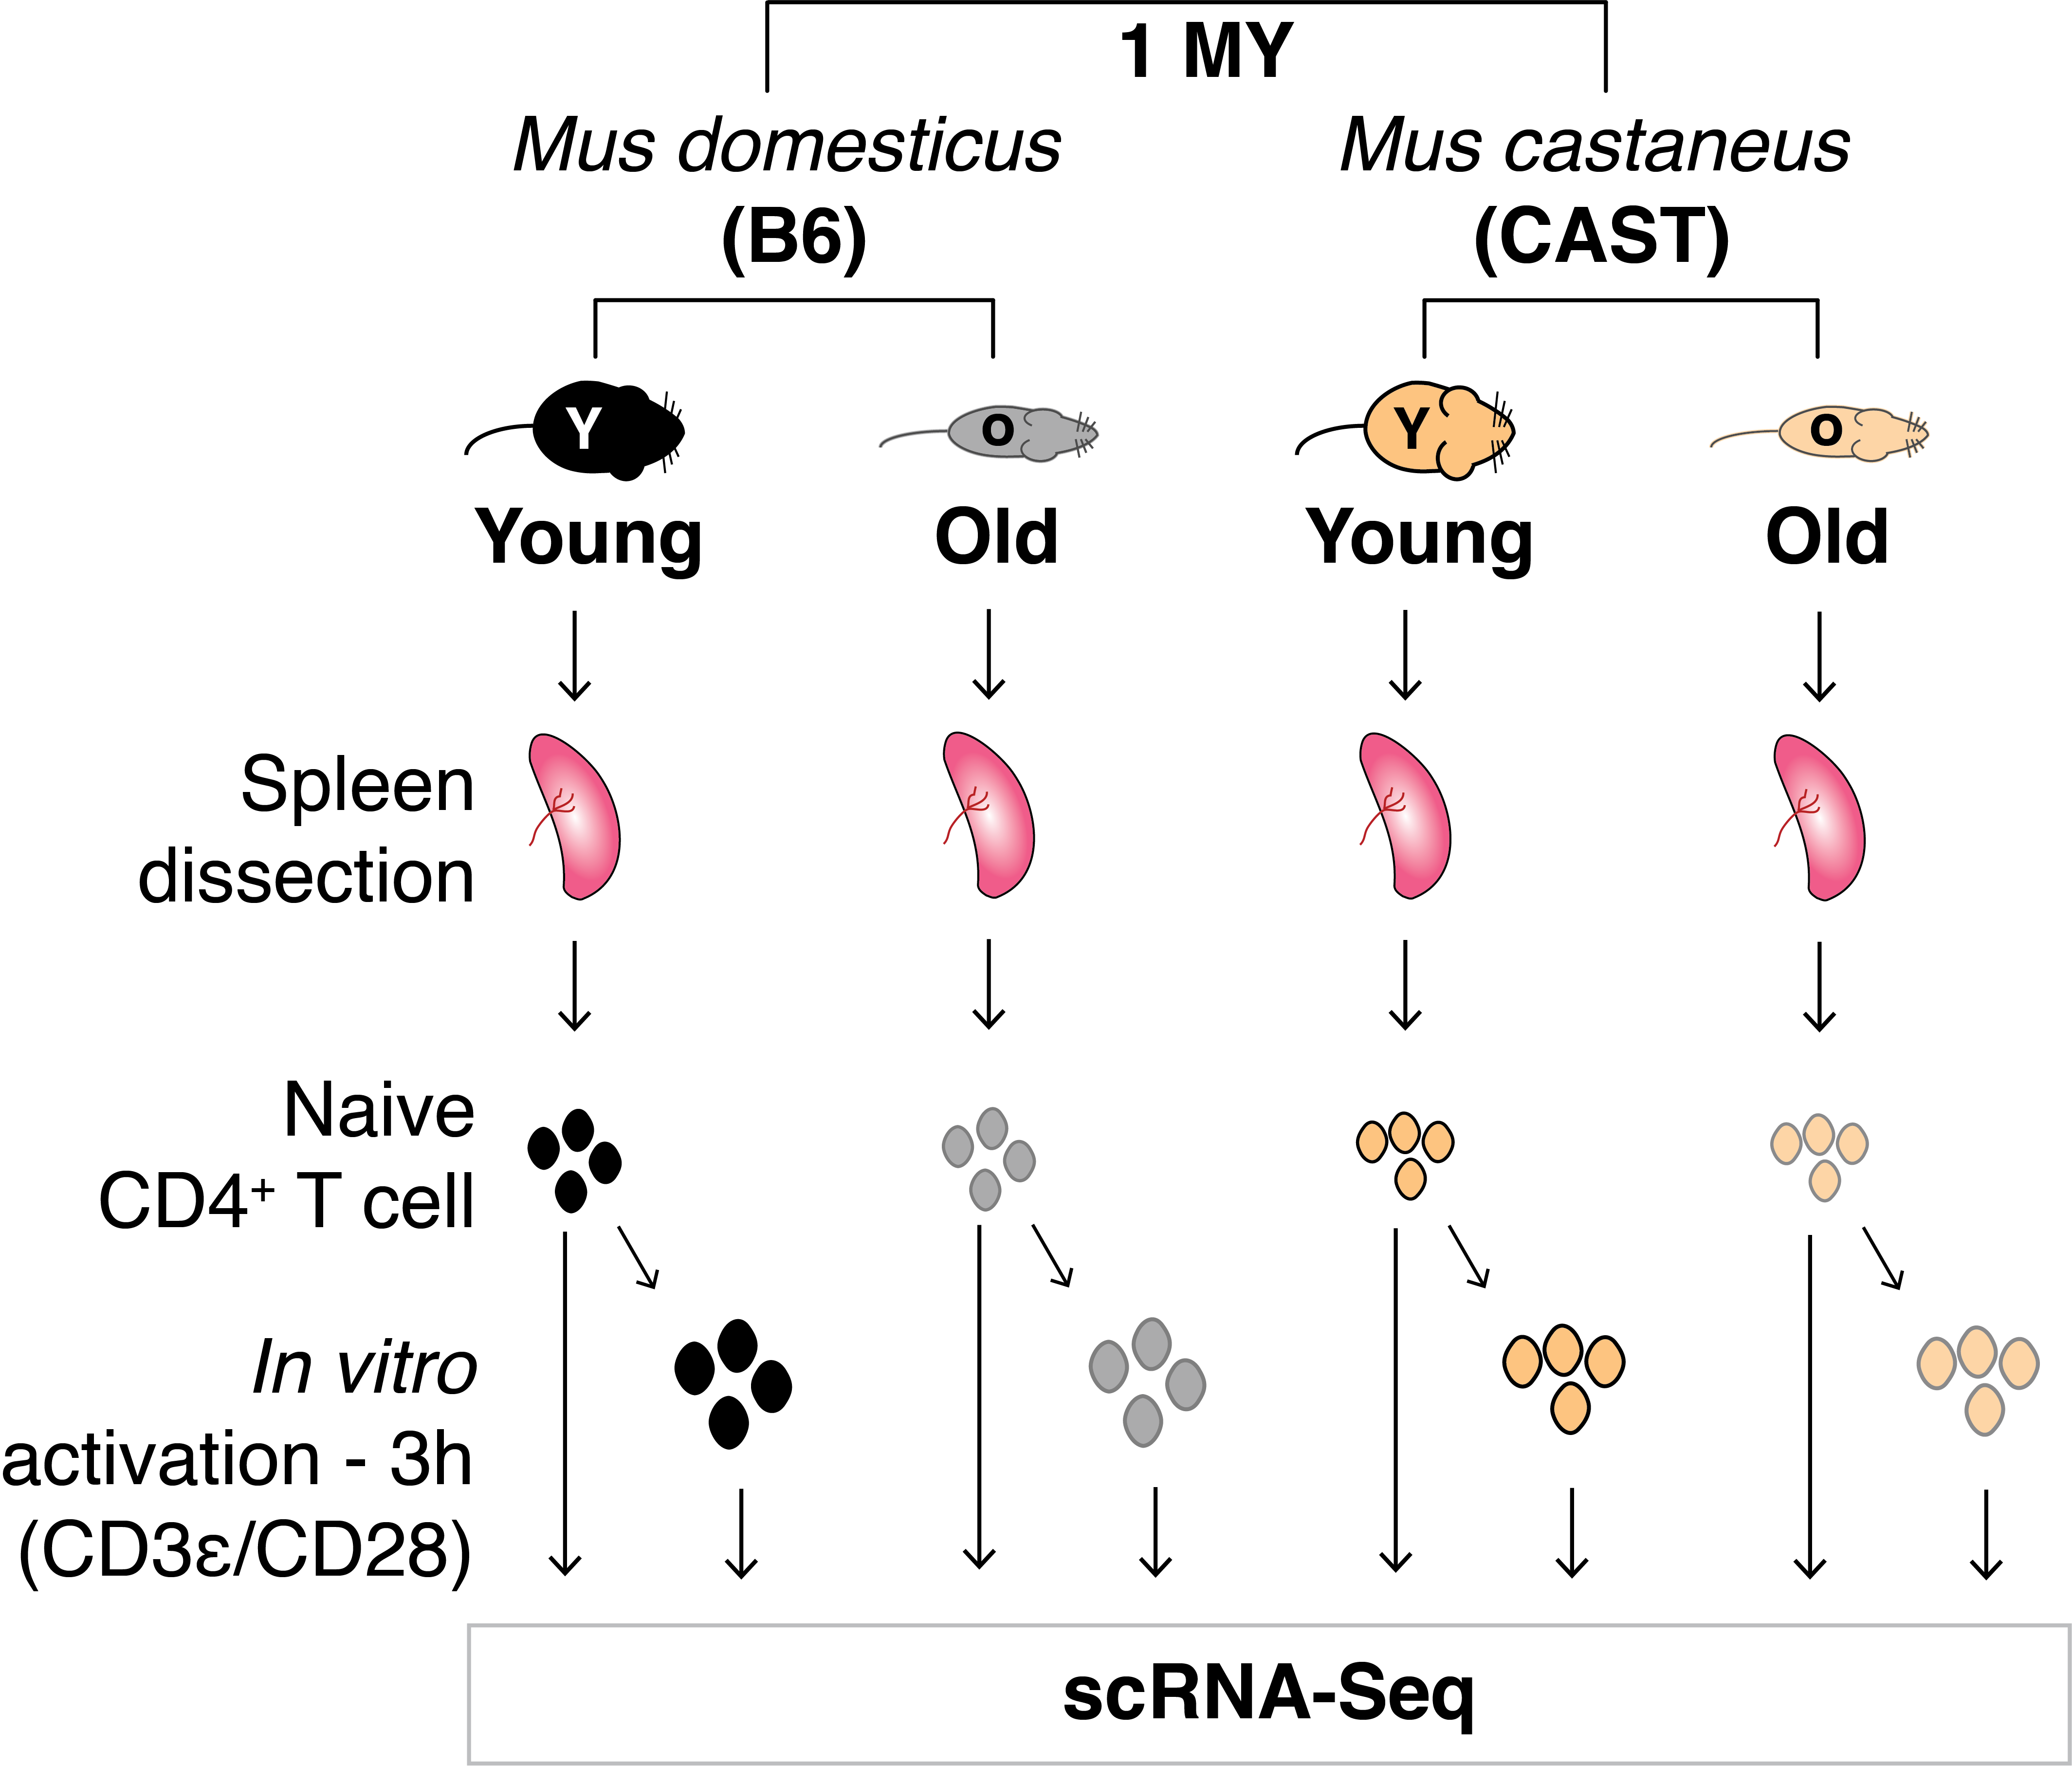
\includegraphics[width=\textwidth]{Fig_1.png}
\caption[Staging of the testicular seminiferous epithelium]{\textbf{Staging of the testicular seminiferous epithelium (full legend on next page).}\\}
\label{fig3:cell_staging}
\end{figure}

\newpage

\captionsetup[figure]{list=no}
\addtocounter{figure}{-1}   
\captionof{figure}{\textbf{Staging of the testicular seminiferous epithelium (continued).}\\
\textbf{(A)} Periodic Acid Schiff (PAS)-stained testis cross-section showing a number of seminiferous tubules at different epithelial stages (displayed as Roman numerals). Within each tubule, the inset circle refers to the corresponding section in (B). Scale bar represents 100 µm; original magnification 200X. \textbf{(B)} Schematic representation of the 12 stages of the seminiferous epithelium in mice. The colour gradient within the circle indicates the differentiation path of germ cells with the layers corresponding to individual cycles of the epithelium. The circle is divided into 12 section, each corresponding to one epithelial stage displaying the characteristic germ cells. Within each section, cells are positioned across the different layers according to their emergence during consecutive cycles, each being 8.6 days apart with more mature cells moving towards the centre.  Cell types are labelled as: A – type A spermatogonia (SG), In – intermediate SG, B – type B SG, Pl – preleptotene spermatocytes (SCs), L – leptotene SCs, Z – zygotene SCs, P – pachytene SCs, D – diplotene SCs, M – metaphase I and II, 1-8 round spermatids, 9-16 elongating spermatids. \textbf{(C)} Higher magnification of two tubules depicted in (A). The PAS-stained cross-sections depict tubules in Stage VII and Stage X, with the different cell layers indicated by coloured lines. Stage VII tubules contain 4 different layers with germ cells from different generations that are approximately 8.6 days apart, whereas Stage X tubules only contain three layers. Each layer contains a certain set of germ cells depending on the epithelial stage. Stage VII contains preleptotene spermatocytes (Pl) in the first layer, pachytene spermatocytes (P) in the second layer, S7 round spermatids (7) in the third layer and S16 elongating spermatids in the fourth innermost layer. Stage X tubules contain leptotene spermatocytes (L) in the first layer, pachytene spermatocytes (P) in the the second layer and only one generation of round-to-elongating spermatids at S10 (10) in the innermost layer. Original magnification 400X.  \\}
\captionsetup[figure]{list=yes}

To fully dissect mouse spermatogenesis, we primarily analysed droplet based single-cell RNA sequencing using the 10X Chromium technology \citep{Zheng2017}. For this, mouse testes were enzymatically dissociated and single-cell suspensions at a concentration of ~300,000 cells/ml was loaded into one channel of the ChromiumTM Single Cell A Chip (10X Genomics), aiming for a recovery of 4000-5000 high-quality cells. Cells were isolated from specifically staged juvenile (between postnatal days 6 and 35) and adult (8-9 weeks) C57BL/6J (B6) mice \textbf{(Table \ref{tab3:QC_scRNAseq})}. To obtain gene-specific transcript counts for droplet based scRNA-Seq, the Cell Ranger \emph{count} function with default settings was used to align and count unique molecular identifiers (UMIs) per sample. This software retains cells with similar UMI distributions \citep{Zheng2017} which we label as "high-quality" transcriptomes. We use this default threshold to obtain high-quality cells with large numbers of UMIs. After merging all samples, we filtered out cells that express less than 1000 genes. Furthermore, we exclude cells with more than 10\% of reads mapping to the mitochondrial genome. \\
Using the Cell Ranger default threshold leads to the exclusion of cells with lower transcriptional complexity. We therefore used the emptyDrops function provided in the \emph{DropletUtils} Bioconductor package \citep{Lun2018} to statistically distinguish empty droplets from genuine cells (controlling the FDR to 1\%). After merging true cells across all samples, we filtered out cells with less than 500 genes expressed. Furthermore, we excluded cells with more than 10\% or mitochondrial genes expressed \textbf{(Table \ref{tab3:QC_scRNAseq})}. The transcriptomes of quality filtered cells were normalized using the scran package \citep{Lun2016pooling}. After quality control and filtering, we retained more than 20,000 high-quality single cells and over 46,000 cells including the once with lower transcriptional complexity \textbf{(Table \ref{tab3:QC_scRNAseq})}. \\
This two-way approach allows us to (i) dissect molecular processes using high-quality cells and capture all testicular cell types, even cells with low transcriptional complexity.\\

Additionally, for juvenile samples, we generated whole-tissue bulk RNA sequencing, as well as mapping chromatin state in purified cell populations using CUT\&{}RUN (Cleavage Under Targets \& Release Using Nuclease) \citep{Skene2018}. With this, we additionally generated 30 bulk RNA-Seq libraries and 8 CUT\&{}RUN libraries.The full experimental set-up can be seen in \textbf{Fig.~\ref{fig3:experimental_design}}.

\begin{figure}[!h]
\centering
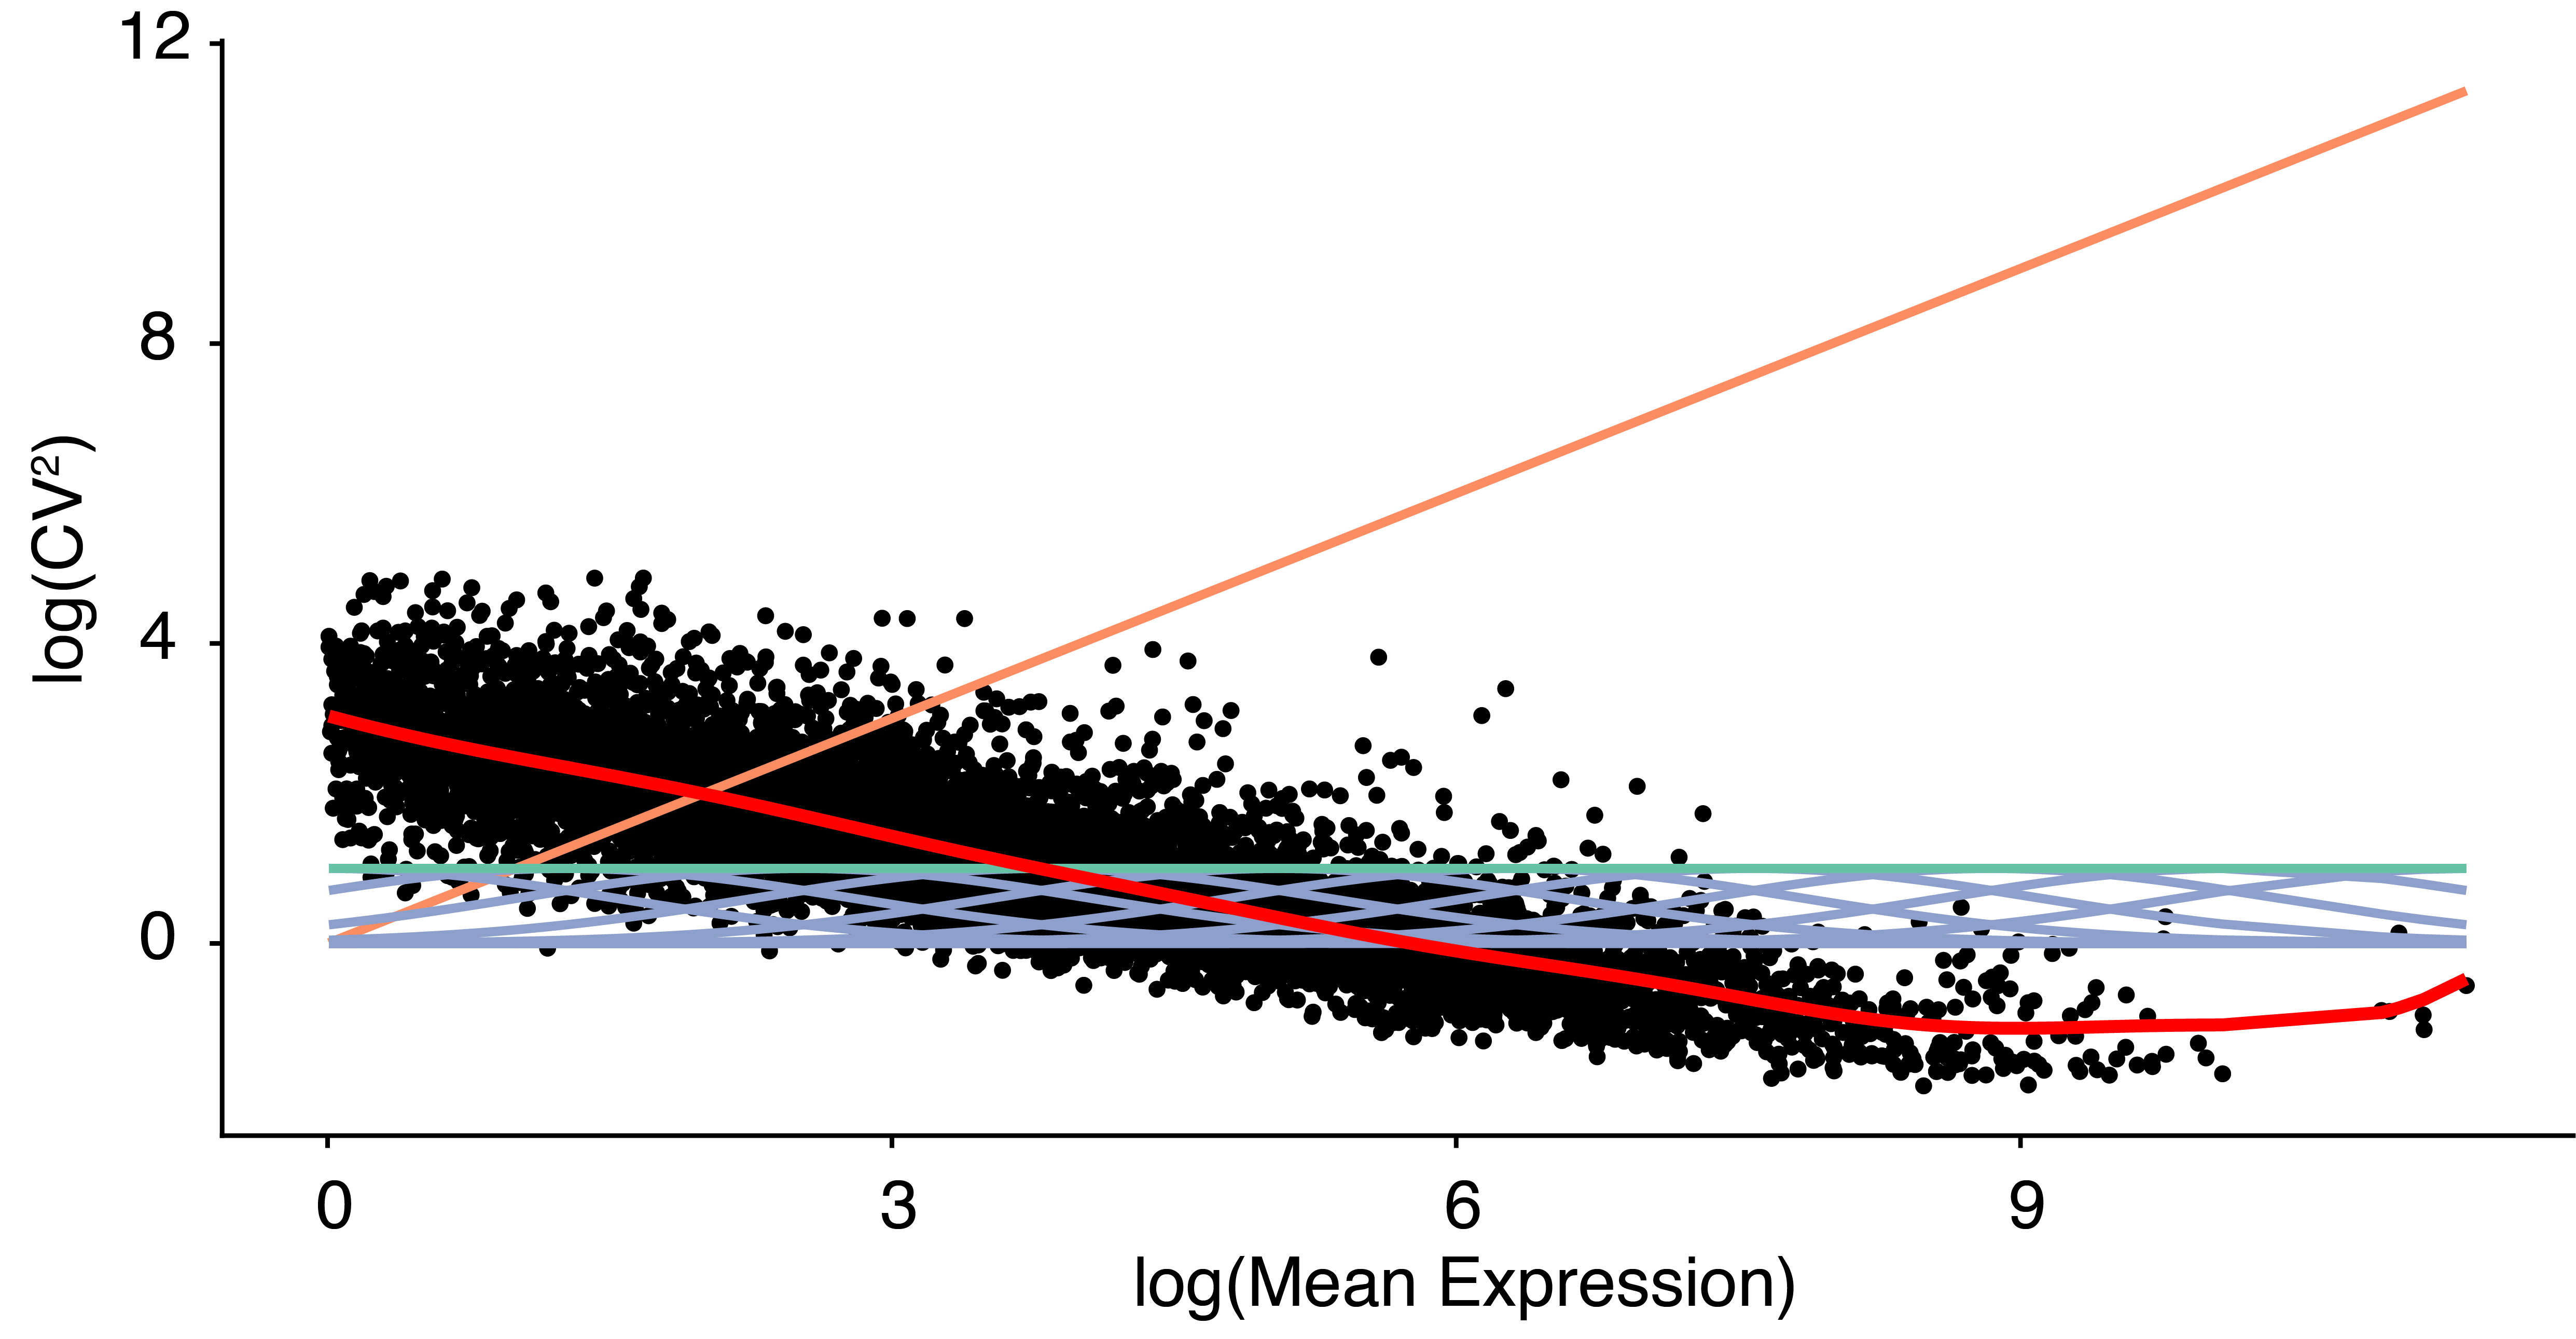
\includegraphics[width=\textwidth]{Fig_2.png}
\caption[Experimental design to dissect mouse spermatogenesis]{\textbf{Experimental design to dissect mouse spermatogenesis.}\\
Overview of the experimental design yielding bulk RNA-Seq, droplet-based scRNA-Seq and chromatin profiling on FACS-purified cells using CUT\&{}RUN from one testis while using the contralateral testis for matched histology.}
\label{fig3:experimental_design}
\end{figure}

To remove batch-specific effects that arise when samples are prepared and sequenced in different experiments \textbf{(Tables \ref{tab3:QC_scRNAseq})}, we used the \emph{mnnCorrect} function implemented in the \emph{scran} package \citep{Haghverdi2018}. We used the top 1000 genes with highest biological variation across all samples as informative genes for batch correction. The \emph{mnnCorrect} function takes transcriptional profiles of cells isolated from adult B6 mice as first input and uses this dataset as reference for cell mapping. This approach maps the juvenile samples onto the adult B6 \textbf{(Fig.~\ref{fig3:cell_types}A)}

\begin{table}[ht	]
\centering
\caption[Quality filtering of scRNAseq data]{\textbf{Quality filtering of scRNAseq data.} \\
Quality metrics of droplet-based scRNA-Seq. Sample: Stage and genotype information for all samples. Library: sample identifier. CellRanger filter: Number of retained cells after default thresholding using the CellRanger counts function.  After quality control: Number of cells obtained after quality control. Assigned Cell Type: Number of cells that fall into annotated clusters (removing outlying cells). EmptyDrops filter: Number of cells retained after using the emptyDrops function controling the FDR to 1\%. EmptyDrops quality control: Number of cells obtained after quality control of the \emph{emptyDrops} filtered cells.}
\label{tab3:QC_scRNAseq}
\begin{tabular}{lllllll}
\toprule
\textbf{Sample} & \textbf{Library} & \textbf{CellRanger} & \textbf{After} & \textbf{Assigned} & \textbf{EmptyDrops} & \textbf{EmptyDrops} \\
& & \textbf{filter} & \textbf{QC} & \textbf{Cell Type} & \textbf{filter} & \textbf{QC} \\
\midrule
B6     & do17815 & 1157              & 1157                  & 1123               & 4467              & 3400                       \\
\midrule
B6     & do17816 & 2198              & 2198                  & 2092               & 6145              & 4603                       \\
\midrule
P10    & do17821 & 3229              & 3213                  & 3212               & 4976              & 4202                       \\
\midrule
P15    & do18195 & 4258              & 4258                  & 4014               & 14050             & 13168                      \\
\midrule
P20    & do17824 & 1775              & 1775                  & 1662               & 9400              & 7491                       \\
\midrule
P25    & do18196 & 4334              & 4334                  & 4130               & 8038              & 6802                       \\
\midrule
P30    & do17825 & 2278              & 2278                  & 2211               & 5393              & 4958                       \\
\midrule
P35    & do17827 & 3160              & 3160                  & 3004               & 49002             & 10683                      \\                 
\bottomrule   
\end{tabular}
\end{table}

To identify cell types across all samples, batch corrected transcriptomes were clustered using a graph-based approach. A shared nearest-neighbour (SNN) graph \citep{Xu2015} was constructed considering 3 shared nearest neighbours using the \emph{buildSNNGraph} function in scran. In the next step, a multi-level modularity optimization algorithm was used to find community structure in the graph \citep{Blondel2008} implemented in \emph{igraph} R package. Cells in small clusters that show unclear identities were excluded from down-stream analysis.\\
We next aimed to annotate clusters based on the expression of marker genes. The adult B6 samples were used to identify marker genes for all germ cell-types present in testes. To this end, we performed differential expression testing across multiple pairwise comparisons. To detect cluster-specific marker genes, the \emph{findMarkers} function implemented in \emph{scran} was used on the log$_2$-transformed normalized counts while providing the cluster labels \textbf{(Fig.~\ref{fig3:cell_types}B)}. \\

On a broad level and by visualizing the expression of detected marker genes, we identified the following cell types: spermatogonia (based on \textit{Dmrt1} expression, \citep{Matson2010}), spermatocytes (\textit{Piwil1}, \citep{Deng2002}), round and elongating spermatids (\textit{Tex21} and \textit{Tnp1}, respectively, \citep{Fujii2002}), as well as the main somatic cell types of the testis, Sertoli (\textit{Cldn11}, \citep{Mazaud-Guittot2010}) and Leydig cells (\textit{Fabp3}, \citep{Oresti2013}) \textbf{(Fig.~\ref{fig3:cell_types}B)}. Using a dimensionality reduction technique for visualization (t-distributed Stochastic Neighbour Embedding; \textbf{Fig.~\ref{fig3:cell_types}C}), the germ cell types from spermatocytes to elongating spermatids formed a continuum, which recapitulated the known developmental trajectory.

\begin{figure}[!h]
\centering
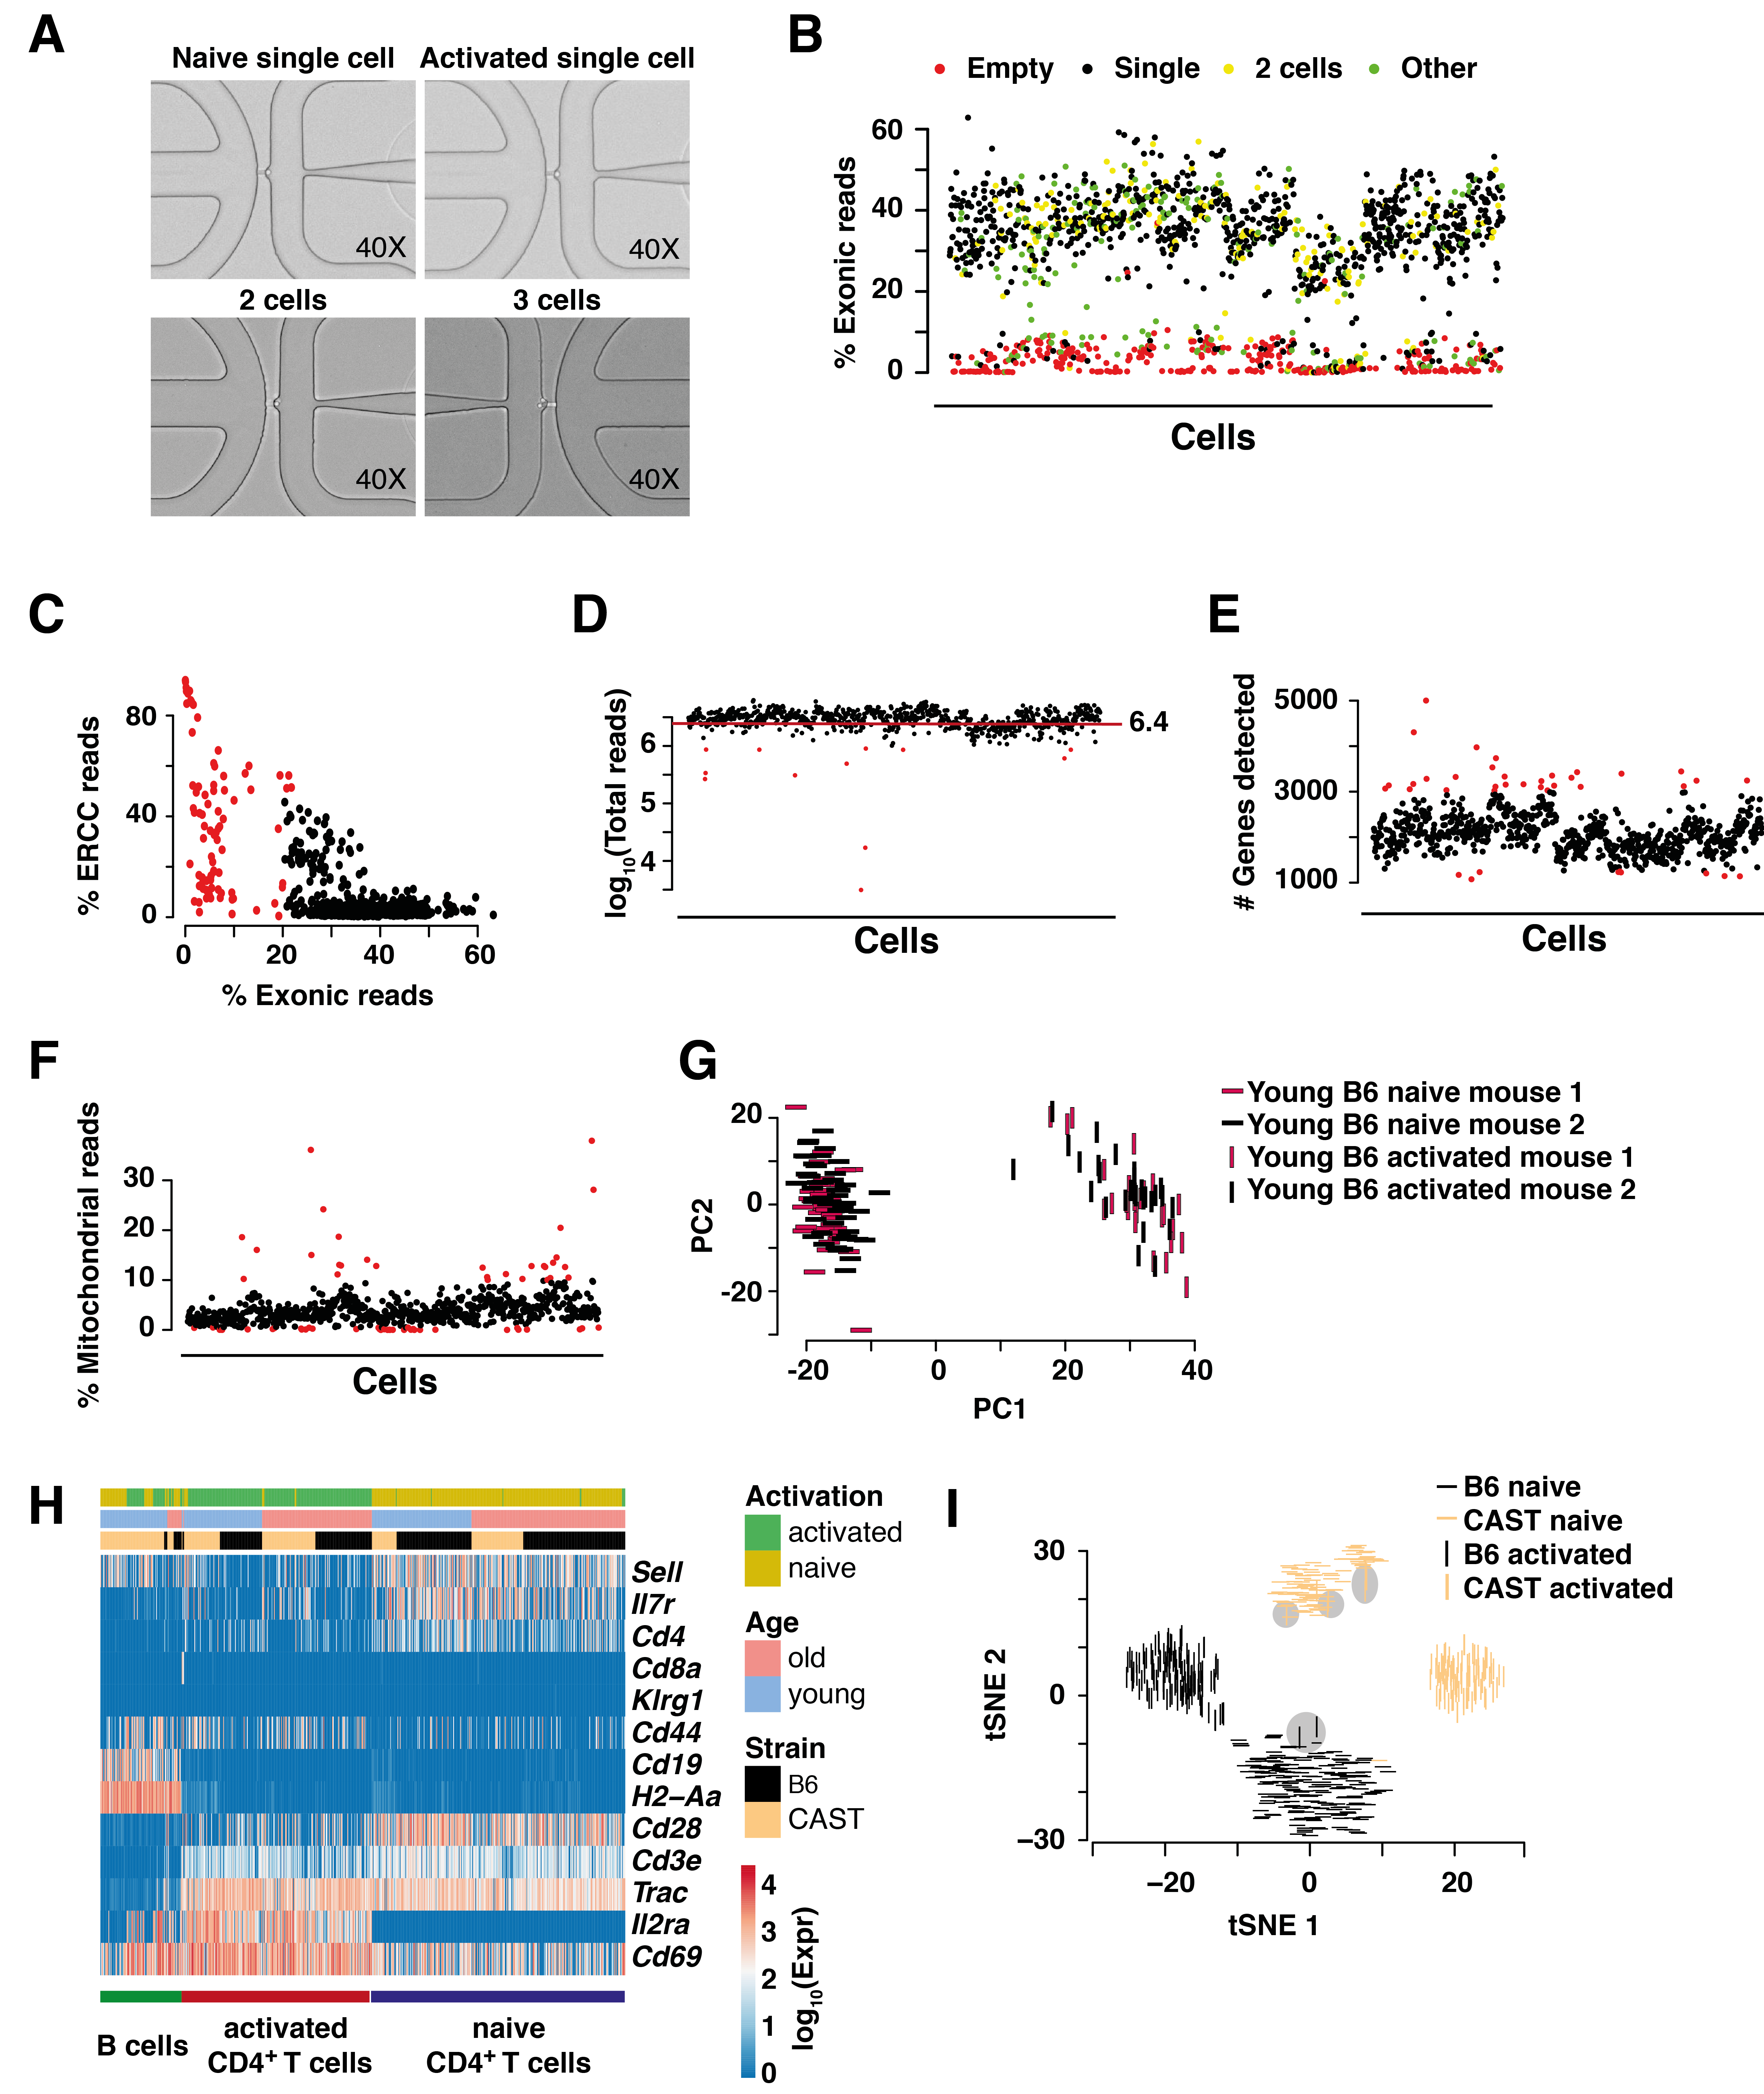
\includegraphics[width=0.8\textwidth]{Fig_3.png}
\caption[Droplet based scRNAseq of mouse spermatogenesis]{\textbf{Single-cell RNA-Seq captures a continuum of germ cell types during adult spermatogenesis.}\\
\textbf{(A)} tSNE representation of juvenile cells that were mapped to cells isolated from adult mice. Grey dots indicate all cells from adult animals that were used as a reference for cell mapping (see Methods). Coloured dots represent cells isolated at each sampled stage during the first wave of spermatogenesis. Clustering has been perfomed across all cells after cell mapping (see Methods). SG: Spermatogonia, M: Meiosis, IL: Imature Leydig, PTM: Peritubular Myoid Cells, EC: Endothelial Cells, tMg: testicular Marcophages. \textbf{(B)} tSNE representation of scRNA-Seq data from adult B6 mice with the colour gradient representing the expression of known marker genes for two somatic cell types and the main germ cell types. The x- and y-axis represent the first and second dimension of tSNE respectively. The colour legend shows log2-transformed, normalized expression counts. \textbf{(E)} Graph-based clustering (see Methods) identifies different sub-stages within major germ cell populations. 
}
\label{fig3:cell_types}
\end{figure}

\section{Developmental staging of mouse spermatogenesis}
\subsection*{Staged developmental mapping of the first wave of spermatogenesis defines germ cell identity}

Historically, sub-staging of the major cell types within the testis was based on changes in nuclear or cellular morphology \citep{Oakberg1956,  Oakberg1956a}. Previous attempts to complement morphology with molecular signatures have been limited to FACS-based and sedimentation assays, where the resolution was unable to differentiate between sub-cell-types \citep{Bastos2005, Gaysinskaya2014, Lam1970, Meistrich1977, Romrell1976, Soumillon2013}. While a mixture of all spermatogenic cell types co-exists in the adult, the first wave of spermatogenesis during juvenile development is more synchronised. Starting around mouse postnatal day P4, spermatogonia begin to differentiate, forming the first generation of spermatocytes as early as P10, round spermatids by P20, and completing the first wave of spermatogenesis with the production of mature spermatozoa between P30 and P35 \textbf{(Fig.~\ref{fig3:1st_wave}A)} \citep{Bellve1977, Janca1986, Nebel1961}.\\
 
We exploited this first spermatogenic wave to generate thousands of high-resolution single-cell transcriptional profiles of morphologically well-defined cell populations. For this, we sampled multiple time points during the first wave to identify the most mature (differentiated) cell types. Based on known sperm developmental transitions, we chose six time points between P10 and P35 from which to generate single-cell RNA-Seq libraries \textbf{(Fig.~\ref{fig3:1st_wave}A)}. For each juvenile experiment, we found that the population of developing germ cells was strongly enriched at the expected developmental stage, as quantified by the percentage of cells in each cell-type cluster \textbf{(Fig.~\ref{fig3:1st_wave}B and C)}. By associating these cell types with the corresponding cell types in the adult trajectory, we unambiguously assigned molecular and histological signatures to cells during adult spermatogenesis.\\

For instance, at P15 the majority of cells are spermatogonia and spermatocytes progressing through the mid-pachytene stage, in accord with the appearance of the sex body \citep{Turner2004}. Interestingly, less mature cell types are also present at this time point (and later time points), supporting recent reports that the first wave of spermatogenesis is less synchronized than previously anticipated \citep{Snyder2010}. At P20, we detect an enrichment for spermatocytes, cells undergoing meiotic cell division, and a small group of early round spermatids. This population structure is in line with matched histology, which shows a large number of tubules in late stages IX-XII and the first occurrence of early round spermatids \citep{Bellve1977}.\\
Spermatids first reach the elongating state between P24 and P26 \citep{Janca1986}. At P25, we observed cells matched to our first ten clusters of spermatids, which we then labelled according to morphologically-defined spermatid substages S1 – S10 \textbf{(Fig.~\ref{fig3:1st_wave}C)}. At P30 and P35, we observed a relatively even distribution of cells across all groups, closely resembling the adult distribution up to S14, indicating that the first wave of spermatogenesis is complete. 

\begin{figure}[!h]
\centering
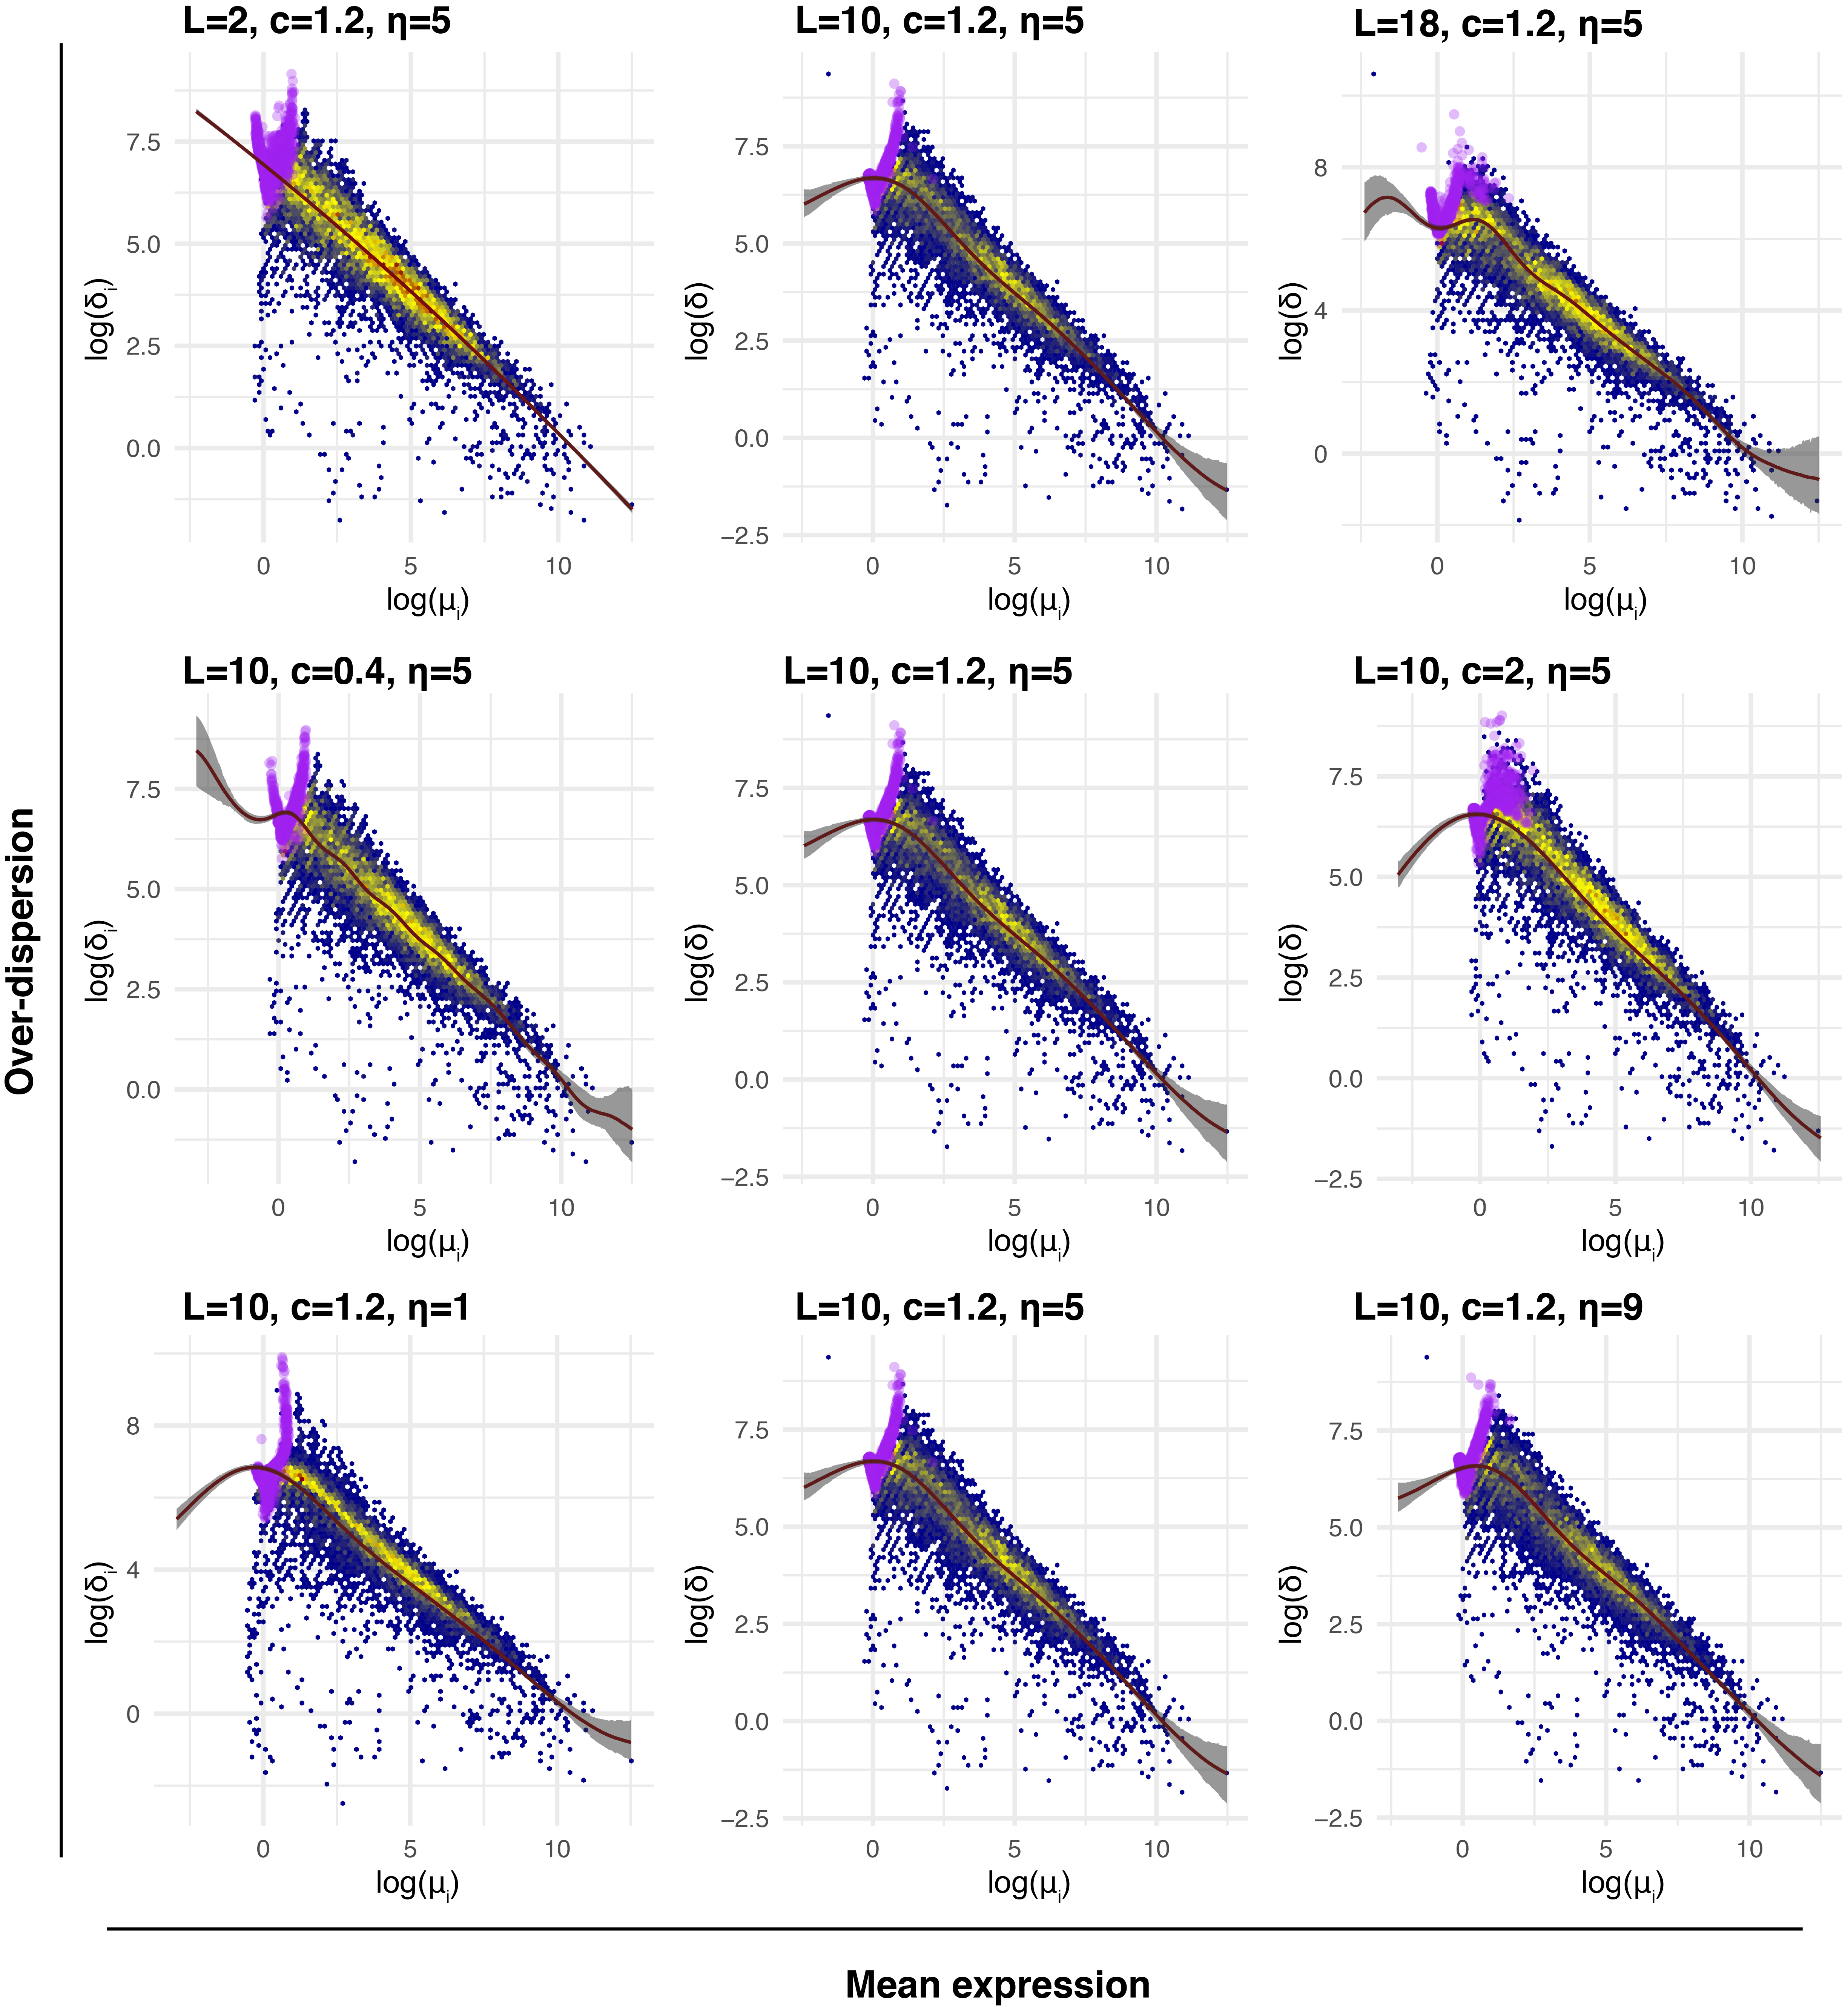
\includegraphics[width=0.85\textwidth]{Fig_4.png}
\caption[Staging of cell types during mouse spermatogenesis]{\textbf{Cell type classification by developmental mapping of time points during the first wave of spermatogenesis (full legend on next page).}}
\label{fig3:1st_wave}
\end{figure}

\newpage

\captionsetup[figure]{list=no}
\addtocounter{figure}{-1}   
\captionof{figure}{\textbf{Cell type classification by developmental mapping of time points during the first wave of spermatogenesis (continued).}\\
\textbf{(A)} Schematic representation of the major germ cell types and their corresponding developmental processes. Spermatogonia differentiate undergoing mitotic cell divisions before forming spermatocytes that divide by meiotic division. Spermatids differentiate throughout spermiogenesis to form mature sperm. The timeline in the lower panel indicates at which point during the first wave of spermatogenesis samples were harvested for the generation of scRNA-Seq (X) or bulk RNA-Seq (B) data. \textbf{(B)} Representative images of seminiferous tubules from PAS-stained tissue cross-sections from animals harvested at different postnatal (P) time points during the first wave of spermatogenesis. The approximate timing of the stage and cycle of the tubule is illustrated below in the form of a circle (see Fig.~\ref{fig3:cell_staging}B). \textbf{(C)} The percentage of cells allocated to each cell cluster for each juvenile and adult sample is represented by the size of squares with the colours corresponding to the clusters depicted in Fig. \ref{fig3:cell_types}C. tSNEs on the right-hand side of each panel (juvenile samples only) illustrate progress through spermatogenesis.  SG – spermatogonia, M – metaphase. \textbf{(D)} Probabilistic mapping of bulk RNA-Seq libraries to the cell clusters identified in the adult scRNA-Seq data using a random forest approach. The colour gradient indicates the probability with which a bulk sample can be assigned to the specific cell cluster.  \\}
\captionsetup[figure]{list=yes}

To further validate the identity of the cell clusters, we used bulk RNA-Seq from testis collected during the first wave of spermatogenesis every two days between P6 and P34 \textbf{(Fig.~\ref{fig3:1st_wave}A)}. We used a regression approach to link the bulk samples to the transcriptomic profiles of single cells. Using the top 50 cluster-specific marker genes for spermatogonia, all spermatocyte groups, all spermatid groups, sertoli and leydig cells, we trained a random forest classifier (implemented in the \emph{randomForest} R package \citep{Liaw2002}) on 2000 cells isolated from adult B6 testes. Model testing was performed on the remaining 1215 cells isolated from adult B6 testes. Prior to training and testing, log$_2$-transformed, normalized counts were scaled by computing the Z score for each gene. Probabilistic prediction was performed using the Z score of log$_2$-transformed, normalized bulk RNA-Seq reads of the input genes. This confirmed that between P6 – P14 spermatogonia and somatic cells show the highest contribution to the transcriptomic profile \textbf{(Fig.~\ref{fig3:1st_wave}D)}. Between P16 and P20 we observed the emergence of spermatocyte-specific gene expression signatures, after which spermatids become the transcriptionally dominant cell type. By P26, spermatids reach the elongating state where transcription is uniformly shut-down due to the beginning of the histone-to-protamine transition \citep{Steger1999}; following this, changes in RNA content are mostly due to degradation. Bulk transcriptional profiles can therefore only be classified up to S10, because transcription is largely inactive thereafter.\\

In sum, by combining transcriptional and histological analyses at specific stages during the first wave of spermatogenesis, we assigned transcriptional profiles to specific, morphologically defined germ cell types.





